% Created by tikzDevice version 0.12.3.2 on 2022-02-15 21:05:12
% !TEX encoding = UTF-8 Unicode
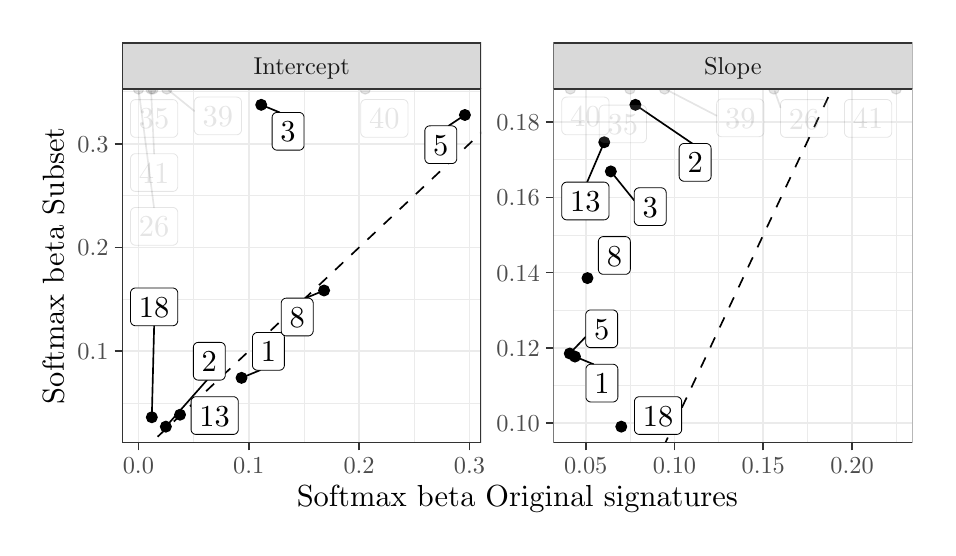
\begin{tikzpicture}[x=1pt,y=1pt]
\definecolor{fillColor}{RGB}{255,255,255}
\path[use as bounding box,fill=fillColor,fill opacity=0.00] (0,0) rectangle (325.21,180.67);
\begin{scope}
\path[clip] (  0.00,  0.00) rectangle (325.21,180.67);
\definecolor{drawColor}{RGB}{255,255,255}
\definecolor{fillColor}{RGB}{255,255,255}

\path[draw=drawColor,line width= 0.6pt,line join=round,line cap=round,fill=fillColor] (  0.00,  0.00) rectangle (325.21,180.68);
\end{scope}
\begin{scope}
\path[clip] ( 34.16, 30.69) rectangle (163.89,158.60);
\definecolor{fillColor}{RGB}{255,255,255}

\path[fill=fillColor] ( 34.16, 30.69) rectangle (163.89,158.60);
\definecolor{drawColor}{gray}{0.92}

\path[draw=drawColor,line width= 0.3pt,line join=round] ( 34.16, 45.05) --
	(163.89, 45.05);

\path[draw=drawColor,line width= 0.3pt,line join=round] ( 34.16, 82.52) --
	(163.89, 82.52);

\path[draw=drawColor,line width= 0.3pt,line join=round] ( 34.16,120.00) --
	(163.89,120.00);

\path[draw=drawColor,line width= 0.3pt,line join=round] ( 34.16,157.47) --
	(163.89,157.47);

\path[draw=drawColor,line width= 0.3pt,line join=round] ( 59.94, 30.69) --
	( 59.94,158.60);

\path[draw=drawColor,line width= 0.3pt,line join=round] ( 99.82, 30.69) --
	( 99.82,158.60);

\path[draw=drawColor,line width= 0.3pt,line join=round] (139.70, 30.69) --
	(139.70,158.60);

\path[draw=drawColor,line width= 0.6pt,line join=round] ( 34.16, 63.79) --
	(163.89, 63.79);

\path[draw=drawColor,line width= 0.6pt,line join=round] ( 34.16,101.26) --
	(163.89,101.26);

\path[draw=drawColor,line width= 0.6pt,line join=round] ( 34.16,138.73) --
	(163.89,138.73);

\path[draw=drawColor,line width= 0.6pt,line join=round] ( 40.00, 30.69) --
	( 40.00,158.60);

\path[draw=drawColor,line width= 0.6pt,line join=round] ( 79.88, 30.69) --
	( 79.88,158.60);

\path[draw=drawColor,line width= 0.6pt,line join=round] (119.76, 30.69) --
	(119.76,158.60);

\path[draw=drawColor,line width= 0.6pt,line join=round] (159.64, 30.69) --
	(159.64,158.60);
\definecolor{drawColor}{RGB}{0,0,0}

\path[draw=drawColor,line width= 0.6pt,dash pattern=on 4pt off 4pt ,line join=round] ( 11.99,  0.00) -- (204.28,180.67);
\definecolor{fillColor}{RGB}{0,0,0}

\path[draw=drawColor,line width= 0.4pt,line join=round,line cap=round,fill=fillColor] ( 77.28, 54.13) circle (  1.96);

\path[draw=drawColor,line width= 0.4pt,line join=round,line cap=round,fill=fillColor] ( 49.93, 36.50) circle (  1.96);

\path[draw=drawColor,line width= 0.4pt,line join=round,line cap=round,fill=fillColor] ( 84.39,152.79) circle (  1.96);

\path[draw=drawColor,line width= 0.4pt,line join=round,line cap=round,fill=fillColor] (157.99,149.12) circle (  1.96);

\path[draw=drawColor,line width= 0.4pt,line join=round,line cap=round,fill=fillColor] (107.11, 85.70) circle (  1.96);

\path[draw=drawColor,line width= 0.4pt,line join=round,line cap=round,fill=fillColor] ( 55.06, 40.81) circle (  1.96);

\path[draw=drawColor,line width= 0.4pt,line join=round,line cap=round,fill=fillColor] ( 44.86, 39.89) circle (  1.96);
\definecolor{drawColor}{RGB}{0,0,0}
\definecolor{fillColor}{RGB}{0,0,0}

\path[draw=drawColor,draw opacity=0.10,line width= 0.4pt,line join=round,line cap=round,fill=fillColor,fill opacity=0.10] ( 40.05,158.60) circle (  1.96);

\path[draw=drawColor,draw opacity=0.10,line width= 0.4pt,line join=round,line cap=round,fill=fillColor,fill opacity=0.10] ( 45.29,158.60) circle (  1.96);

\path[draw=drawColor,draw opacity=0.10,line width= 0.4pt,line join=round,line cap=round,fill=fillColor,fill opacity=0.10] ( 50.28,158.60) circle (  1.96);

\path[draw=drawColor,draw opacity=0.10,line width= 0.4pt,line join=round,line cap=round,fill=fillColor,fill opacity=0.10] (121.97,158.60) circle (  1.96);

\path[draw=drawColor,draw opacity=0.10,line width= 0.4pt,line join=round,line cap=round,fill=fillColor,fill opacity=0.10] ( 44.56,158.60) circle (  1.96);
\end{scope}
\begin{scope}
\path[clip] ( 34.16, 30.69) rectangle (163.89,158.60);
\definecolor{drawColor}{RGB}{0,0,0}

\path[draw=drawColor,line width= 0.6pt,line join=round,line cap=round] ( 83.99, 56.90) -- ( 78.15, 54.49);

\path[draw=drawColor,line width= 0.6pt,line join=round,line cap=round] ( 64.78, 53.32) -- ( 50.55, 37.20);

\path[draw=drawColor,line width= 0.6pt,line join=round,line cap=round] ( 91.09,150.04) -- ( 85.26,152.43);

\path[draw=drawColor,line width= 0.6pt,line join=round,line cap=round] (152.09,145.20) -- (157.22,148.61);

\path[draw=drawColor,line width= 0.6pt,line join=round,line cap=round] (100.40, 82.93) -- (106.24, 85.34);

\path[draw=drawColor,line width= 0.6pt,line join=round,line cap=round] ( 45.70, 72.97) -- ( 44.88, 40.81);
\definecolor{drawColor}{RGB}{0,0,0}

\path[draw=drawColor,draw opacity=0.10,line width= 0.6pt,line join=round,line cap=round] ( 45.65,115.69) -- ( 40.17,157.69);

\path[draw=drawColor,draw opacity=0.10,line width= 0.6pt,line join=round,line cap=round] ( 60.20,150.56) -- ( 51.00,158.02);

\path[draw=drawColor,draw opacity=0.10,line width= 0.6pt,line join=round,line cap=round] ( 45.70,135.13) -- ( 44.60,157.68);
\definecolor{drawColor}{RGB}{0,0,0}
\definecolor{fillColor}{RGB}{255,255,255}

\path[draw=drawColor,line width= 0.3pt,line join=round,line cap=round,fill=fillColor] ( 83.03, 56.90) --
	( 90.96, 56.90) --
	( 90.89, 56.90) --
	( 91.18, 56.91) --
	( 91.46, 56.97) --
	( 91.73, 57.07) --
	( 91.99, 57.22) --
	( 92.21, 57.40) --
	( 92.40, 57.62) --
	( 92.56, 57.86) --
	( 92.67, 58.13) --
	( 92.74, 58.41) --
	( 92.77, 58.70) --
	( 92.77, 58.70) --
	( 92.77, 68.72) --
	( 92.77, 68.72) --
	( 92.74, 69.00) --
	( 92.67, 69.29) --
	( 92.56, 69.55) --
	( 92.40, 69.80) --
	( 92.21, 70.02) --
	( 91.99, 70.20) --
	( 91.73, 70.35) --
	( 91.46, 70.45) --
	( 91.18, 70.51) --
	( 90.96, 70.52) --
	( 83.03, 70.52) --
	( 83.25, 70.51) --
	( 82.96, 70.52) --
	( 82.67, 70.49) --
	( 82.39, 70.40) --
	( 82.13, 70.28) --
	( 81.89, 70.11) --
	( 81.68, 69.91) --
	( 81.50, 69.68) --
	( 81.37, 69.42) --
	( 81.28, 69.15) --
	( 81.23, 68.86) --
	( 81.23, 68.72) --
	( 81.23, 58.70) --
	( 81.23, 58.85) --
	( 81.23, 58.56) --
	( 81.28, 58.27) --
	( 81.37, 57.99) --
	( 81.50, 57.74) --
	( 81.68, 57.50) --
	( 81.89, 57.30) --
	( 82.13, 57.14) --
	( 82.39, 57.01) --
	( 82.67, 56.93) --
	( 82.96, 56.90) --
	cycle;
\end{scope}
\begin{scope}
\path[clip] ( 34.16, 30.69) rectangle (163.89,158.60);
\definecolor{drawColor}{RGB}{0,0,0}

\node[text=drawColor,anchor=base,inner sep=0pt, outer sep=0pt, scale=  1.10] at ( 87.00, 59.91) {1};
\definecolor{fillColor}{RGB}{255,255,255}

\path[draw=drawColor,line width= 0.3pt,line join=round,line cap=round,fill=fillColor] ( 61.68, 53.32) --
	( 69.60, 53.32) --
	( 69.53, 53.32) --
	( 69.82, 53.33) --
	( 70.11, 53.39) --
	( 70.38, 53.49) --
	( 70.63, 53.64) --
	( 70.86, 53.82) --
	( 71.05, 54.04) --
	( 71.20, 54.29) --
	( 71.32, 54.55) --
	( 71.39, 54.84) --
	( 71.41, 55.13) --
	( 71.41, 55.13) --
	( 71.41, 65.14) --
	( 71.41, 65.14) --
	( 71.39, 65.43) --
	( 71.32, 65.71) --
	( 71.20, 65.98) --
	( 71.05, 66.22) --
	( 70.86, 66.44) --
	( 70.63, 66.62) --
	( 70.38, 66.77) --
	( 70.11, 66.87) --
	( 69.82, 66.93) --
	( 69.60, 66.94) --
	( 61.68, 66.94) --
	( 61.89, 66.93) --
	( 61.60, 66.94) --
	( 61.32, 66.91) --
	( 61.04, 66.83) --
	( 60.77, 66.70) --
	( 60.53, 66.54) --
	( 60.32, 66.34) --
	( 60.15, 66.10) --
	( 60.01, 65.85) --
	( 59.92, 65.57) --
	( 59.88, 65.28) --
	( 59.87, 65.14) --
	( 59.87, 55.13) --
	( 59.88, 55.27) --
	( 59.88, 54.98) --
	( 59.92, 54.69) --
	( 60.01, 54.42) --
	( 60.15, 54.16) --
	( 60.32, 53.93) --
	( 60.53, 53.73) --
	( 60.77, 53.56) --
	( 61.04, 53.44) --
	( 61.32, 53.35) --
	( 61.60, 53.32) --
	cycle;
\end{scope}
\begin{scope}
\path[clip] ( 34.16, 30.69) rectangle (163.89,158.60);
\definecolor{drawColor}{RGB}{0,0,0}

\node[text=drawColor,anchor=base,inner sep=0pt, outer sep=0pt, scale=  1.10] at ( 65.64, 56.33) {2};
\definecolor{fillColor}{RGB}{255,255,255}

\path[draw=drawColor,line width= 0.3pt,line join=round,line cap=round,fill=fillColor] ( 90.14,136.41) --
	( 98.06,136.41) --
	( 97.99,136.41) --
	( 98.28,136.42) --
	( 98.57,136.48) --
	( 98.84,136.58) --
	( 99.09,136.73) --
	( 99.32,136.91) --
	( 99.51,137.13) --
	( 99.66,137.38) --
	( 99.78,137.64) --
	( 99.85,137.93) --
	( 99.87,138.22) --
	( 99.87,138.22) --
	( 99.87,148.23) --
	( 99.87,148.23) --
	( 99.85,148.52) --
	( 99.78,148.80) --
	( 99.66,149.07) --
	( 99.51,149.31) --
	( 99.32,149.53) --
	( 99.09,149.72) --
	( 98.84,149.86) --
	( 98.57,149.96) --
	( 98.28,150.02) --
	( 98.06,150.04) --
	( 90.14,150.04) --
	( 90.35,150.02) --
	( 90.06,150.03) --
	( 89.77,150.00) --
	( 89.50,149.92) --
	( 89.23,149.79) --
	( 88.99,149.63) --
	( 88.78,149.43) --
	( 88.61,149.19) --
	( 88.47,148.94) --
	( 88.38,148.66) --
	( 88.34,148.37) --
	( 88.33,148.23) --
	( 88.33,138.22) --
	( 88.34,138.36) --
	( 88.34,138.07) --
	( 88.38,137.78) --
	( 88.47,137.51) --
	( 88.61,137.25) --
	( 88.78,137.02) --
	( 88.99,136.82) --
	( 89.23,136.65) --
	( 89.50,136.53) --
	( 89.77,136.45) --
	( 90.06,136.41) --
	cycle;
\end{scope}
\begin{scope}
\path[clip] ( 34.16, 30.69) rectangle (163.89,158.60);
\definecolor{drawColor}{RGB}{0,0,0}

\node[text=drawColor,anchor=base,inner sep=0pt, outer sep=0pt, scale=  1.10] at ( 94.10,139.42) {3};
\definecolor{fillColor}{RGB}{255,255,255}

\path[draw=drawColor,line width= 0.3pt,line join=round,line cap=round,fill=fillColor] (145.33,131.57) --
	(153.26,131.57) --
	(153.19,131.57) --
	(153.48,131.58) --
	(153.76,131.64) --
	(154.04,131.74) --
	(154.29,131.89) --
	(154.51,132.07) --
	(154.71,132.29) --
	(154.86,132.54) --
	(154.98,132.80) --
	(155.04,133.09) --
	(155.07,133.38) --
	(155.07,133.38) --
	(155.07,143.39) --
	(155.07,143.39) --
	(155.04,143.68) --
	(154.98,143.96) --
	(154.86,144.23) --
	(154.71,144.47) --
	(154.51,144.69) --
	(154.29,144.88) --
	(154.04,145.02) --
	(153.76,145.12) --
	(153.48,145.18) --
	(153.26,145.20) --
	(145.33,145.20) --
	(145.55,145.18) --
	(145.26,145.19) --
	(144.97,145.16) --
	(144.69,145.08) --
	(144.43,144.95) --
	(144.19,144.79) --
	(143.98,144.59) --
	(143.81,144.36) --
	(143.67,144.10) --
	(143.58,143.82) --
	(143.53,143.53) --
	(143.53,143.39) --
	(143.53,133.38) --
	(143.53,133.52) --
	(143.53,133.23) --
	(143.58,132.94) --
	(143.67,132.67) --
	(143.81,132.41) --
	(143.98,132.18) --
	(144.19,131.98) --
	(144.43,131.81) --
	(144.69,131.69) --
	(144.97,131.61) --
	(145.26,131.57) --
	cycle;
\end{scope}
\begin{scope}
\path[clip] ( 34.16, 30.69) rectangle (163.89,158.60);
\definecolor{drawColor}{RGB}{0,0,0}

\node[text=drawColor,anchor=base,inner sep=0pt, outer sep=0pt, scale=  1.10] at (149.30,134.58) {5};
\definecolor{fillColor}{RGB}{255,255,255}

\path[draw=drawColor,line width= 0.3pt,line join=round,line cap=round,fill=fillColor] ( 93.43, 69.30) --
	(101.36, 69.30) --
	(101.29, 69.30) --
	(101.58, 69.31) --
	(101.86, 69.37) --
	(102.13, 69.47) --
	(102.39, 69.62) --
	(102.61, 69.80) --
	(102.80, 70.02) --
	(102.96, 70.27) --
	(103.07, 70.53) --
	(103.14, 70.82) --
	(103.17, 71.11) --
	(103.17, 71.11) --
	(103.17, 81.12) --
	(103.17, 81.12) --
	(103.14, 81.41) --
	(103.07, 81.69) --
	(102.96, 81.96) --
	(102.80, 82.20) --
	(102.61, 82.42) --
	(102.39, 82.61) --
	(102.13, 82.75) --
	(101.86, 82.85) --
	(101.58, 82.91) --
	(101.36, 82.93) --
	( 93.43, 82.93) --
	( 93.65, 82.91) --
	( 93.36, 82.92) --
	( 93.07, 82.89) --
	( 92.79, 82.81) --
	( 92.53, 82.68) --
	( 92.29, 82.52) --
	( 92.08, 82.32) --
	( 91.90, 82.09) --
	( 91.77, 81.83) --
	( 91.68, 81.55) --
	( 91.63, 81.26) --
	( 91.62, 81.12) --
	( 91.62, 71.11) --
	( 91.63, 71.25) --
	( 91.63, 70.96) --
	( 91.68, 70.67) --
	( 91.77, 70.40) --
	( 91.90, 70.14) --
	( 92.08, 69.91) --
	( 92.29, 69.71) --
	( 92.53, 69.54) --
	( 92.79, 69.42) --
	( 93.07, 69.34) --
	( 93.36, 69.30) --
	cycle;
\end{scope}
\begin{scope}
\path[clip] ( 34.16, 30.69) rectangle (163.89,158.60);
\definecolor{drawColor}{RGB}{0,0,0}

\node[text=drawColor,anchor=base,inner sep=0pt, outer sep=0pt, scale=  1.10] at ( 97.39, 72.31) {8};
\definecolor{fillColor}{RGB}{255,255,255}

\path[draw=drawColor,line width= 0.3pt,line join=round,line cap=round,fill=fillColor] ( 60.85, 33.70) --
	( 74.30, 33.70) --
	( 74.23, 33.70) --
	( 74.52, 33.71) --
	( 74.80, 33.77) --
	( 75.07, 33.87) --
	( 75.33, 34.02) --
	( 75.55, 34.20) --
	( 75.74, 34.42) --
	( 75.90, 34.66) --
	( 76.01, 34.93) --
	( 76.08, 35.21) --
	( 76.11, 35.50) --
	( 76.11, 35.50) --
	( 76.11, 45.52) --
	( 76.11, 45.52) --
	( 76.08, 45.81) --
	( 76.01, 46.09) --
	( 75.90, 46.36) --
	( 75.74, 46.60) --
	( 75.55, 46.82) --
	( 75.33, 47.00) --
	( 75.07, 47.15) --
	( 74.80, 47.25) --
	( 74.52, 47.31) --
	( 74.30, 47.32) --
	( 60.85, 47.32) --
	( 61.07, 47.31) --
	( 60.78, 47.32) --
	( 60.49, 47.29) --
	( 60.21, 47.21) --
	( 59.95, 47.08) --
	( 59.71, 46.92) --
	( 59.50, 46.71) --
	( 59.33, 46.48) --
	( 59.19, 46.22) --
	( 59.10, 45.95) --
	( 59.05, 45.66) --
	( 59.05, 45.52) --
	( 59.05, 35.50) --
	( 59.05, 35.65) --
	( 59.05, 35.36) --
	( 59.10, 35.07) --
	( 59.19, 34.80) --
	( 59.33, 34.54) --
	( 59.50, 34.31) --
	( 59.71, 34.10) --
	( 59.95, 33.94) --
	( 60.21, 33.81) --
	( 60.49, 33.73) --
	( 60.78, 33.70) --
	cycle;
\end{scope}
\begin{scope}
\path[clip] ( 34.16, 30.69) rectangle (163.89,158.60);
\definecolor{drawColor}{RGB}{0,0,0}

\node[text=drawColor,anchor=base,inner sep=0pt, outer sep=0pt, scale=  1.10] at ( 67.58, 36.71) {13};
\definecolor{fillColor}{RGB}{255,255,255}

\path[draw=drawColor,line width= 0.3pt,line join=round,line cap=round,fill=fillColor] ( 38.97, 72.97) --
	( 52.42, 72.97) --
	( 52.35, 72.97) --
	( 52.64, 72.98) --
	( 52.92, 73.04) --
	( 53.19, 73.14) --
	( 53.45, 73.29) --
	( 53.67, 73.47) --
	( 53.86, 73.69) --
	( 54.02, 73.94) --
	( 54.13, 74.20) --
	( 54.20, 74.49) --
	( 54.23, 74.78) --
	( 54.23, 74.78) --
	( 54.23, 84.79) --
	( 54.23, 84.79) --
	( 54.20, 85.08) --
	( 54.13, 85.36) --
	( 54.02, 85.63) --
	( 53.86, 85.87) --
	( 53.67, 86.09) --
	( 53.45, 86.27) --
	( 53.19, 86.42) --
	( 52.92, 86.52) --
	( 52.64, 86.58) --
	( 52.42, 86.59) --
	( 38.97, 86.59) --
	( 39.19, 86.58) --
	( 38.90, 86.59) --
	( 38.61, 86.56) --
	( 38.33, 86.48) --
	( 38.07, 86.35) --
	( 37.83, 86.19) --
	( 37.62, 85.99) --
	( 37.45, 85.75) --
	( 37.31, 85.50) --
	( 37.22, 85.22) --
	( 37.17, 84.93) --
	( 37.17, 84.79) --
	( 37.17, 74.78) --
	( 37.17, 74.92) --
	( 37.17, 74.63) --
	( 37.22, 74.34) --
	( 37.31, 74.07) --
	( 37.45, 73.81) --
	( 37.62, 73.58) --
	( 37.83, 73.38) --
	( 38.07, 73.21) --
	( 38.33, 73.09) --
	( 38.61, 73.01) --
	( 38.90, 72.97) --
	cycle;
\end{scope}
\begin{scope}
\path[clip] ( 34.16, 30.69) rectangle (163.89,158.60);
\definecolor{drawColor}{RGB}{0,0,0}

\node[text=drawColor,anchor=base,inner sep=0pt, outer sep=0pt, scale=  1.10] at ( 45.70, 75.98) {18};
\definecolor{drawColor}{RGB}{0,0,0}
\definecolor{fillColor}{RGB}{255,255,255}

\path[draw=drawColor,draw opacity=0.10,line width= 0.3pt,line join=round,line cap=round,fill=fillColor,fill opacity=0.10] ( 38.97,102.06) --
	( 52.42,102.06) --
	( 52.35,102.06) --
	( 52.64,102.08) --
	( 52.92,102.13) --
	( 53.19,102.24) --
	( 53.45,102.38) --
	( 53.67,102.57) --
	( 53.86,102.78) --
	( 54.02,103.03) --
	( 54.13,103.30) --
	( 54.20,103.58) --
	( 54.23,103.87) --
	( 54.23,103.87) --
	( 54.23,113.88) --
	( 54.23,113.88) --
	( 54.20,114.17) --
	( 54.13,114.45) --
	( 54.02,114.72) --
	( 53.86,114.97) --
	( 53.67,115.19) --
	( 53.45,115.37) --
	( 53.19,115.51) --
	( 52.92,115.62) --
	( 52.64,115.68) --
	( 52.42,115.69) --
	( 38.97,115.69) --
	( 39.19,115.68) --
	( 38.90,115.69) --
	( 38.61,115.65) --
	( 38.33,115.57) --
	( 38.07,115.45) --
	( 37.83,115.28) --
	( 37.62,115.08) --
	( 37.45,114.85) --
	( 37.31,114.59) --
	( 37.22,114.31) --
	( 37.17,114.03) --
	( 37.17,113.88) --
	( 37.17,103.87) --
	( 37.17,104.02) --
	( 37.17,103.72) --
	( 37.22,103.44) --
	( 37.31,103.16) --
	( 37.45,102.90) --
	( 37.62,102.67) --
	( 37.83,102.47) --
	( 38.07,102.31) --
	( 38.33,102.18) --
	( 38.61,102.10) --
	( 38.90,102.06) --
	cycle;
\end{scope}
\begin{scope}
\path[clip] ( 34.16, 30.69) rectangle (163.89,158.60);
\definecolor{drawColor}{RGB}{0,0,0}

\node[text=drawColor,text opacity=0.10,anchor=base,inner sep=0pt, outer sep=0pt, scale=  1.10] at ( 45.70,105.07) {26};
\definecolor{fillColor}{RGB}{255,255,255}

\path[draw=drawColor,draw opacity=0.10,line width= 0.3pt,line join=round,line cap=round,fill=fillColor,fill opacity=0.10] ( 38.97,141.05) --
	( 52.42,141.05) --
	( 52.35,141.05) --
	( 52.64,141.06) --
	( 52.92,141.12) --
	( 53.19,141.22) --
	( 53.45,141.37) --
	( 53.67,141.55) --
	( 53.86,141.77) --
	( 54.02,142.01) --
	( 54.13,142.28) --
	( 54.20,142.56) --
	( 54.23,142.85) --
	( 54.23,142.85) --
	( 54.23,152.86) --
	( 54.23,152.86) --
	( 54.20,153.15) --
	( 54.13,153.44) --
	( 54.02,153.70) --
	( 53.86,153.95) --
	( 53.67,154.17) --
	( 53.45,154.35) --
	( 53.19,154.50) --
	( 52.92,154.60) --
	( 52.64,154.66) --
	( 52.42,154.67) --
	( 38.97,154.67) --
	( 39.19,154.66) --
	( 38.90,154.67) --
	( 38.61,154.64) --
	( 38.33,154.55) --
	( 38.07,154.43) --
	( 37.83,154.26) --
	( 37.62,154.06) --
	( 37.45,153.83) --
	( 37.31,153.57) --
	( 37.22,153.30) --
	( 37.17,153.01) --
	( 37.17,152.86) --
	( 37.17,142.85) --
	( 37.17,143.00) --
	( 37.17,142.71) --
	( 37.22,142.42) --
	( 37.31,142.14) --
	( 37.45,141.89) --
	( 37.62,141.65) --
	( 37.83,141.45) --
	( 38.07,141.29) --
	( 38.33,141.16) --
	( 38.61,141.08) --
	( 38.90,141.05) --
	cycle;
\end{scope}
\begin{scope}
\path[clip] ( 34.16, 30.69) rectangle (163.89,158.60);
\definecolor{drawColor}{RGB}{0,0,0}

\node[text=drawColor,text opacity=0.10,anchor=base,inner sep=0pt, outer sep=0pt, scale=  1.10] at ( 45.70,144.06) {35};
\definecolor{fillColor}{RGB}{255,255,255}

\path[draw=drawColor,draw opacity=0.10,line width= 0.3pt,line join=round,line cap=round,fill=fillColor,fill opacity=0.10] ( 62.01,141.97) --
	( 75.45,141.97) --
	( 75.38,141.97) --
	( 75.67,141.98) --
	( 75.96,142.04) --
	( 76.23,142.14) --
	( 76.48,142.29) --
	( 76.71,142.47) --
	( 76.90,142.69) --
	( 77.05,142.93) --
	( 77.17,143.20) --
	( 77.24,143.48) --
	( 77.26,143.77) --
	( 77.26,143.77) --
	( 77.26,153.79) --
	( 77.26,153.79) --
	( 77.24,154.08) --
	( 77.17,154.36) --
	( 77.05,154.63) --
	( 76.90,154.87) --
	( 76.71,155.09) --
	( 76.48,155.27) --
	( 76.23,155.42) --
	( 75.96,155.52) --
	( 75.67,155.58) --
	( 75.45,155.59) --
	( 62.01,155.59) --
	( 62.23,155.58) --
	( 61.94,155.59) --
	( 61.65,155.56) --
	( 61.37,155.47) --
	( 61.10,155.35) --
	( 60.87,155.19) --
	( 60.66,154.98) --
	( 60.48,154.75) --
	( 60.35,154.49) --
	( 60.25,154.22) --
	( 60.21,153.93) --
	( 60.20,153.79) --
	( 60.20,143.77) --
	( 60.21,143.92) --
	( 60.21,143.63) --
	( 60.25,143.34) --
	( 60.35,143.06) --
	( 60.48,142.81) --
	( 60.66,142.57) --
	( 60.87,142.37) --
	( 61.10,142.21) --
	( 61.37,142.08) --
	( 61.65,142.00) --
	( 61.94,141.97) --
	cycle;
\end{scope}
\begin{scope}
\path[clip] ( 34.16, 30.69) rectangle (163.89,158.60);
\definecolor{drawColor}{RGB}{0,0,0}

\node[text=drawColor,text opacity=0.10,anchor=base,inner sep=0pt, outer sep=0pt, scale=  1.10] at ( 68.73,144.98) {39};
\definecolor{fillColor}{RGB}{255,255,255}

\path[draw=drawColor,draw opacity=0.10,line width= 0.3pt,line join=round,line cap=round,fill=fillColor,fill opacity=0.10] (122.17,141.07) --
	(135.62,141.07) --
	(135.55,141.07) --
	(135.84,141.08) --
	(136.12,141.14) --
	(136.39,141.25) --
	(136.65,141.39) --
	(136.87,141.58) --
	(137.06,141.79) --
	(137.22,142.04) --
	(137.33,142.31) --
	(137.40,142.59) --
	(137.43,142.88) --
	(137.43,142.88) --
	(137.43,152.89) --
	(137.43,152.89) --
	(137.40,153.18) --
	(137.33,153.46) --
	(137.22,153.73) --
	(137.06,153.98) --
	(136.87,154.19) --
	(136.65,154.38) --
	(136.39,154.52) --
	(136.12,154.63) --
	(135.84,154.68) --
	(135.62,154.70) --
	(122.17,154.70) --
	(122.39,154.68) --
	(122.10,154.70) --
	(121.81,154.66) --
	(121.53,154.58) --
	(121.27,154.46) --
	(121.03,154.29) --
	(120.82,154.09) --
	(120.65,153.86) --
	(120.51,153.60) --
	(120.42,153.32) --
	(120.37,153.04) --
	(120.37,152.89) --
	(120.37,142.88) --
	(120.37,143.02) --
	(120.37,142.73) --
	(120.42,142.45) --
	(120.51,142.17) --
	(120.65,141.91) --
	(120.82,141.68) --
	(121.03,141.48) --
	(121.27,141.31) --
	(121.53,141.19) --
	(121.81,141.11) --
	(122.10,141.07) --
	cycle;
\end{scope}
\begin{scope}
\path[clip] ( 34.16, 30.69) rectangle (163.89,158.60);
\definecolor{drawColor}{RGB}{0,0,0}

\node[text=drawColor,text opacity=0.10,anchor=base,inner sep=0pt, outer sep=0pt, scale=  1.10] at (128.90,144.08) {40};
\definecolor{fillColor}{RGB}{255,255,255}

\path[draw=drawColor,draw opacity=0.10,line width= 0.3pt,line join=round,line cap=round,fill=fillColor,fill opacity=0.10] ( 38.97,121.51) --
	( 52.42,121.51) --
	( 52.35,121.51) --
	( 52.64,121.52) --
	( 52.92,121.58) --
	( 53.19,121.68) --
	( 53.45,121.83) --
	( 53.67,122.01) --
	( 53.86,122.23) --
	( 54.02,122.47) --
	( 54.13,122.74) --
	( 54.20,123.02) --
	( 54.23,123.31) --
	( 54.23,123.31) --
	( 54.23,133.33) --
	( 54.23,133.33) --
	( 54.20,133.62) --
	( 54.13,133.90) --
	( 54.02,134.17) --
	( 53.86,134.41) --
	( 53.67,134.63) --
	( 53.45,134.81) --
	( 53.19,134.96) --
	( 52.92,135.06) --
	( 52.64,135.12) --
	( 52.42,135.13) --
	( 38.97,135.13) --
	( 39.19,135.12) --
	( 38.90,135.13) --
	( 38.61,135.10) --
	( 38.33,135.02) --
	( 38.07,134.89) --
	( 37.83,134.73) --
	( 37.62,134.52) --
	( 37.45,134.29) --
	( 37.31,134.03) --
	( 37.22,133.76) --
	( 37.17,133.47) --
	( 37.17,133.33) --
	( 37.17,123.31) --
	( 37.17,123.46) --
	( 37.17,123.17) --
	( 37.22,122.88) --
	( 37.31,122.61) --
	( 37.45,122.35) --
	( 37.62,122.12) --
	( 37.83,121.91) --
	( 38.07,121.75) --
	( 38.33,121.62) --
	( 38.61,121.54) --
	( 38.90,121.51) --
	cycle;
\end{scope}
\begin{scope}
\path[clip] ( 34.16, 30.69) rectangle (163.89,158.60);
\definecolor{drawColor}{RGB}{0,0,0}

\node[text=drawColor,text opacity=0.10,anchor=base,inner sep=0pt, outer sep=0pt, scale=  1.10] at ( 45.70,124.52) {41};
\definecolor{drawColor}{gray}{0.20}

\path[draw=drawColor,line width= 0.6pt,line join=round,line cap=round] ( 34.16, 30.69) rectangle (163.89,158.60);
\end{scope}
\begin{scope}
\path[clip] (189.98, 30.69) rectangle (319.71,158.60);
\definecolor{fillColor}{RGB}{255,255,255}

\path[fill=fillColor] (189.98, 30.69) rectangle (319.71,158.60);
\definecolor{drawColor}{gray}{0.92}

\path[draw=drawColor,line width= 0.3pt,line join=round] (189.98, 51.31) --
	(319.71, 51.31);

\path[draw=drawColor,line width= 0.3pt,line join=round] (189.98, 78.53) --
	(319.71, 78.53);

\path[draw=drawColor,line width= 0.3pt,line join=round] (189.98,105.75) --
	(319.71,105.75);

\path[draw=drawColor,line width= 0.3pt,line join=round] (189.98,132.98) --
	(319.71,132.98);

\path[draw=drawColor,line width= 0.3pt,line join=round] (217.69, 30.69) --
	(217.69,158.60);

\path[draw=drawColor,line width= 0.3pt,line join=round] (249.77, 30.69) --
	(249.77,158.60);

\path[draw=drawColor,line width= 0.3pt,line join=round] (281.85, 30.69) --
	(281.85,158.60);

\path[draw=drawColor,line width= 0.3pt,line join=round] (313.94, 30.69) --
	(313.94,158.60);

\path[draw=drawColor,line width= 0.6pt,line join=round] (189.98, 37.70) --
	(319.71, 37.70);

\path[draw=drawColor,line width= 0.6pt,line join=round] (189.98, 64.92) --
	(319.71, 64.92);

\path[draw=drawColor,line width= 0.6pt,line join=round] (189.98, 92.14) --
	(319.71, 92.14);

\path[draw=drawColor,line width= 0.6pt,line join=round] (189.98,119.36) --
	(319.71,119.36);

\path[draw=drawColor,line width= 0.6pt,line join=round] (189.98,146.59) --
	(319.71,146.59);

\path[draw=drawColor,line width= 0.6pt,line join=round] (201.65, 30.69) --
	(201.65,158.60);

\path[draw=drawColor,line width= 0.6pt,line join=round] (233.73, 30.69) --
	(233.73,158.60);

\path[draw=drawColor,line width= 0.6pt,line join=round] (265.81, 30.69) --
	(265.81,158.60);

\path[draw=drawColor,line width= 0.6pt,line join=round] (297.89, 30.69) --
	(297.89,158.60);
\definecolor{drawColor}{RGB}{0,0,0}

\path[draw=drawColor,line width= 0.6pt,dash pattern=on 4pt off 4pt ,line join=round] (215.96,  0.00) -- (301.13,180.67);
\definecolor{fillColor}{RGB}{0,0,0}

\path[draw=drawColor,line width= 0.4pt,line join=round,line cap=round,fill=fillColor] (197.77, 61.82) circle (  1.96);

\path[draw=drawColor,line width= 0.4pt,line join=round,line cap=round,fill=fillColor] (219.60,152.79) circle (  1.96);

\path[draw=drawColor,line width= 0.4pt,line join=round,line cap=round,fill=fillColor] (210.72,128.73) circle (  1.96);

\path[draw=drawColor,line width= 0.4pt,line join=round,line cap=round,fill=fillColor] (195.88, 62.93) circle (  1.96);

\path[draw=drawColor,line width= 0.4pt,line join=round,line cap=round,fill=fillColor] (202.28, 90.18) circle (  1.96);

\path[draw=drawColor,line width= 0.4pt,line join=round,line cap=round,fill=fillColor] (208.34,139.27) circle (  1.96);

\path[draw=drawColor,line width= 0.4pt,line join=round,line cap=round,fill=fillColor] (214.50, 36.50) circle (  1.96);
\definecolor{drawColor}{RGB}{0,0,0}
\definecolor{fillColor}{RGB}{0,0,0}

\path[draw=drawColor,draw opacity=0.10,line width= 0.4pt,line join=round,line cap=round,fill=fillColor,fill opacity=0.10] (269.66,158.60) circle (  1.96);

\path[draw=drawColor,draw opacity=0.10,line width= 0.4pt,line join=round,line cap=round,fill=fillColor,fill opacity=0.10] (217.63,158.60) circle (  1.96);

\path[draw=drawColor,draw opacity=0.10,line width= 0.4pt,line join=round,line cap=round,fill=fillColor,fill opacity=0.10] (230.16,158.60) circle (  1.96);

\path[draw=drawColor,draw opacity=0.10,line width= 0.4pt,line join=round,line cap=round,fill=fillColor,fill opacity=0.10] (196.08,158.60) circle (  1.96);

\path[draw=drawColor,draw opacity=0.10,line width= 0.4pt,line join=round,line cap=round,fill=fillColor,fill opacity=0.10] (313.82,158.60) circle (  1.96);
\end{scope}
\begin{scope}
\path[clip] (189.98, 30.69) rectangle (319.71,158.60);
\definecolor{drawColor}{RGB}{0,0,0}

\path[draw=drawColor,line width= 0.6pt,line join=round,line cap=round] (204.48, 59.04) -- (198.63, 61.46);

\path[draw=drawColor,line width= 0.6pt,line join=round,line cap=round] (240.16,138.81) -- (220.37,152.26);

\path[draw=drawColor,line width= 0.6pt,line join=round,line cap=round] (219.18,118.23) -- (211.30,128.01);

\path[draw=drawColor,line width= 0.6pt,line join=round,line cap=round] (201.64, 68.95) -- (196.52, 63.60);

\path[draw=drawColor,line width= 0.6pt,line join=round,line cap=round] (202.16,124.85) -- (207.98,138.42);
\definecolor{drawColor}{RGB}{0,0,0}

\path[draw=drawColor,draw opacity=0.10,line width= 0.6pt,line join=round,line cap=round] (272.04,151.83) -- (269.97,157.73);

\path[draw=drawColor,draw opacity=0.10,line width= 0.6pt,line join=round,line cap=round] (248.96,148.86) -- (230.99,158.17);
\definecolor{drawColor}{RGB}{0,0,0}
\definecolor{fillColor}{RGB}{255,255,255}

\path[draw=drawColor,line width= 0.3pt,line join=round,line cap=round,fill=fillColor] (203.52, 45.42) --
	(211.45, 45.42) --
	(211.38, 45.42) --
	(211.67, 45.43) --
	(211.95, 45.49) --
	(212.23, 45.59) --
	(212.48, 45.74) --
	(212.70, 45.92) --
	(212.90, 46.14) --
	(213.05, 46.39) --
	(213.17, 46.65) --
	(213.24, 46.93) --
	(213.26, 47.22) --
	(213.26, 47.22) --
	(213.26, 57.24) --
	(213.26, 57.24) --
	(213.24, 57.53) --
	(213.17, 57.81) --
	(213.05, 58.08) --
	(212.90, 58.32) --
	(212.70, 58.54) --
	(212.48, 58.72) --
	(212.23, 58.87) --
	(211.95, 58.97) --
	(211.67, 59.03) --
	(211.45, 59.04) --
	(203.52, 59.04) --
	(203.74, 59.03) --
	(203.45, 59.04) --
	(203.16, 59.01) --
	(202.88, 58.93) --
	(202.62, 58.80) --
	(202.38, 58.64) --
	(202.17, 58.44) --
	(202.00, 58.20) --
	(201.86, 57.95) --
	(201.77, 57.67) --
	(201.72, 57.38) --
	(201.72, 57.24) --
	(201.72, 47.22) --
	(201.72, 47.37) --
	(201.72, 47.08) --
	(201.77, 46.79) --
	(201.86, 46.52) --
	(202.00, 46.26) --
	(202.17, 46.03) --
	(202.38, 45.83) --
	(202.62, 45.66) --
	(202.88, 45.54) --
	(203.16, 45.45) --
	(203.45, 45.42) --
	cycle;
\end{scope}
\begin{scope}
\path[clip] (189.98, 30.69) rectangle (319.71,158.60);
\definecolor{drawColor}{RGB}{0,0,0}

\node[text=drawColor,anchor=base,inner sep=0pt, outer sep=0pt, scale=  1.10] at (207.49, 48.43) {1};
\definecolor{fillColor}{RGB}{255,255,255}

\path[draw=drawColor,line width= 0.3pt,line join=round,line cap=round,fill=fillColor] (237.22,125.19) --
	(245.15,125.19) --
	(245.07,125.19) --
	(245.36,125.20) --
	(245.65,125.26) --
	(245.92,125.36) --
	(246.17,125.51) --
	(246.40,125.69) --
	(246.59,125.91) --
	(246.75,126.15) --
	(246.86,126.42) --
	(246.93,126.70) --
	(246.95,126.99) --
	(246.95,126.99) --
	(246.95,137.01) --
	(246.95,137.01) --
	(246.93,137.30) --
	(246.86,137.58) --
	(246.75,137.85) --
	(246.59,138.09) --
	(246.40,138.31) --
	(246.17,138.49) --
	(245.92,138.64) --
	(245.65,138.74) --
	(245.36,138.80) --
	(245.15,138.81) --
	(237.22,138.81) --
	(237.44,138.80) --
	(237.15,138.81) --
	(236.86,138.78) --
	(236.58,138.70) --
	(236.31,138.57) --
	(236.08,138.41) --
	(235.87,138.20) --
	(235.69,137.97) --
	(235.56,137.71) --
	(235.46,137.44) --
	(235.42,137.15) --
	(235.41,137.01) --
	(235.41,126.99) --
	(235.42,127.14) --
	(235.42,126.85) --
	(235.46,126.56) --
	(235.56,126.29) --
	(235.69,126.03) --
	(235.87,125.80) --
	(236.08,125.59) --
	(236.31,125.43) --
	(236.58,125.30) --
	(236.86,125.22) --
	(237.15,125.19) --
	cycle;
\end{scope}
\begin{scope}
\path[clip] (189.98, 30.69) rectangle (319.71,158.60);
\definecolor{drawColor}{RGB}{0,0,0}

\node[text=drawColor,anchor=base,inner sep=0pt, outer sep=0pt, scale=  1.10] at (241.18,128.20) {2};
\definecolor{fillColor}{RGB}{255,255,255}

\path[draw=drawColor,line width= 0.3pt,line join=round,line cap=round,fill=fillColor] (220.98,109.18) --
	(228.91,109.18) --
	(228.84,109.18) --
	(229.13,109.19) --
	(229.41,109.25) --
	(229.69,109.35) --
	(229.94,109.50) --
	(230.16,109.68) --
	(230.36,109.90) --
	(230.51,110.15) --
	(230.63,110.41) --
	(230.69,110.70) --
	(230.72,110.99) --
	(230.72,110.99) --
	(230.72,121.00) --
	(230.72,121.00) --
	(230.69,121.29) --
	(230.63,121.57) --
	(230.51,121.84) --
	(230.36,122.08) --
	(230.16,122.30) --
	(229.94,122.49) --
	(229.69,122.63) --
	(229.41,122.73) --
	(229.13,122.79) --
	(228.91,122.81) --
	(220.98,122.81) --
	(221.20,122.79) --
	(220.91,122.80) --
	(220.62,122.77) --
	(220.34,122.69) --
	(220.08,122.56) --
	(219.84,122.40) --
	(219.63,122.20) --
	(219.46,121.96) --
	(219.32,121.71) --
	(219.23,121.43) --
	(219.18,121.14) --
	(219.18,121.00) --
	(219.18,110.99) --
	(219.18,111.13) --
	(219.18,110.84) --
	(219.23,110.55) --
	(219.32,110.28) --
	(219.46,110.02) --
	(219.63,109.79) --
	(219.84,109.59) --
	(220.08,109.42) --
	(220.34,109.30) --
	(220.62,109.22) --
	(220.91,109.18) --
	cycle;
\end{scope}
\begin{scope}
\path[clip] (189.98, 30.69) rectangle (319.71,158.60);
\definecolor{drawColor}{RGB}{0,0,0}

\node[text=drawColor,anchor=base,inner sep=0pt, outer sep=0pt, scale=  1.10] at (224.95,112.19) {3};
\definecolor{fillColor}{RGB}{255,255,255}

\path[draw=drawColor,line width= 0.3pt,line join=round,line cap=round,fill=fillColor] (203.45, 65.04) --
	(211.38, 65.04) --
	(211.31, 65.05) --
	(211.60, 65.06) --
	(211.88, 65.12) --
	(212.15, 65.22) --
	(212.40, 65.36) --
	(212.63, 65.55) --
	(212.82, 65.77) --
	(212.98, 66.01) --
	(213.09, 66.28) --
	(213.16, 66.56) --
	(213.19, 66.85) --
	(213.19, 66.85) --
	(213.19, 76.86) --
	(213.19, 76.86) --
	(213.16, 77.15) --
	(213.09, 77.44) --
	(212.98, 77.70) --
	(212.82, 77.95) --
	(212.63, 78.17) --
	(212.40, 78.35) --
	(212.15, 78.50) --
	(211.88, 78.60) --
	(211.60, 78.66) --
	(211.38, 78.67) --
	(203.45, 78.67) --
	(203.67, 78.66) --
	(203.38, 78.67) --
	(203.09, 78.63) --
	(202.81, 78.55) --
	(202.55, 78.43) --
	(202.31, 78.26) --
	(202.10, 78.06) --
	(201.92, 77.83) --
	(201.79, 77.57) --
	(201.70, 77.30) --
	(201.65, 77.01) --
	(201.64, 76.86) --
	(201.64, 66.85) --
	(201.65, 67.00) --
	(201.65, 66.71) --
	(201.70, 66.42) --
	(201.79, 66.14) --
	(201.92, 65.89) --
	(202.10, 65.65) --
	(202.31, 65.45) --
	(202.55, 65.29) --
	(202.81, 65.16) --
	(203.09, 65.08) --
	(203.38, 65.05) --
	cycle;
\end{scope}
\begin{scope}
\path[clip] (189.98, 30.69) rectangle (319.71,158.60);
\definecolor{drawColor}{RGB}{0,0,0}

\node[text=drawColor,anchor=base,inner sep=0pt, outer sep=0pt, scale=  1.10] at (207.41, 68.06) {5};
\definecolor{fillColor}{RGB}{255,255,255}

\path[draw=drawColor,line width= 0.3pt,line join=round,line cap=round,fill=fillColor] (208.03, 91.54) --
	(215.96, 91.54) --
	(215.89, 91.54) --
	(216.18, 91.55) --
	(216.46, 91.61) --
	(216.74, 91.72) --
	(216.99, 91.86) --
	(217.21, 92.05) --
	(217.41, 92.26) --
	(217.56, 92.51) --
	(217.68, 92.78) --
	(217.75, 93.06) --
	(217.77, 93.35) --
	(217.77, 93.35) --
	(217.77,103.36) --
	(217.77,103.36) --
	(217.75,103.65) --
	(217.68,103.93) --
	(217.56,104.20) --
	(217.41,104.45) --
	(217.21,104.66) --
	(216.99,104.85) --
	(216.74,104.99) --
	(216.46,105.10) --
	(216.18,105.15) --
	(215.96,105.17) --
	(208.03,105.17) --
	(208.25,105.15) --
	(207.96,105.17) --
	(207.67,105.13) --
	(207.39,105.05) --
	(207.13,104.93) --
	(206.89,104.76) --
	(206.68,104.56) --
	(206.51,104.33) --
	(206.37,104.07) --
	(206.28,103.79) --
	(206.23,103.51) --
	(206.23,103.36) --
	(206.23, 93.35) --
	(206.23, 93.49) --
	(206.23, 93.20) --
	(206.28, 92.92) --
	(206.37, 92.64) --
	(206.51, 92.38) --
	(206.68, 92.15) --
	(206.89, 91.95) --
	(207.13, 91.78) --
	(207.39, 91.66) --
	(207.67, 91.58) --
	(207.96, 91.54) --
	cycle;
\end{scope}
\begin{scope}
\path[clip] (189.98, 30.69) rectangle (319.71,158.60);
\definecolor{drawColor}{RGB}{0,0,0}

\node[text=drawColor,anchor=base,inner sep=0pt, outer sep=0pt, scale=  1.10] at (212.00, 94.55) {8};
\definecolor{fillColor}{RGB}{255,255,255}

\path[draw=drawColor,line width= 0.3pt,line join=round,line cap=round,fill=fillColor] (194.80,111.22) --
	(208.25,111.22) --
	(208.17,111.22) --
	(208.46,111.24) --
	(208.75,111.29) --
	(209.02,111.40) --
	(209.27,111.54) --
	(209.50,111.73) --
	(209.69,111.94) --
	(209.85,112.19) --
	(209.96,112.46) --
	(210.03,112.74) --
	(210.05,113.03) --
	(210.05,113.03) --
	(210.05,123.04) --
	(210.05,123.04) --
	(210.03,123.33) --
	(209.96,123.61) --
	(209.85,123.88) --
	(209.69,124.13) --
	(209.50,124.34) --
	(209.27,124.53) --
	(209.02,124.67) --
	(208.75,124.78) --
	(208.46,124.84) --
	(208.25,124.85) --
	(194.80,124.85) --
	(195.02,124.84) --
	(194.73,124.85) --
	(194.44,124.81) --
	(194.16,124.73) --
	(193.90,124.61) --
	(193.66,124.44) --
	(193.45,124.24) --
	(193.27,124.01) --
	(193.14,123.75) --
	(193.04,123.47) --
	(193.00,123.19) --
	(192.99,123.04) --
	(192.99,113.03) --
	(193.00,113.17) --
	(193.00,112.88) --
	(193.04,112.60) --
	(193.14,112.32) --
	(193.27,112.06) --
	(193.45,111.83) --
	(193.66,111.63) --
	(193.90,111.46) --
	(194.16,111.34) --
	(194.44,111.26) --
	(194.73,111.22) --
	cycle;
\end{scope}
\begin{scope}
\path[clip] (189.98, 30.69) rectangle (319.71,158.60);
\definecolor{drawColor}{RGB}{0,0,0}

\node[text=drawColor,anchor=base,inner sep=0pt, outer sep=0pt, scale=  1.10] at (201.52,114.23) {13};
\definecolor{fillColor}{RGB}{255,255,255}

\path[draw=drawColor,line width= 0.3pt,line join=round,line cap=round,fill=fillColor] (221.06, 33.70) --
	(234.50, 33.70) --
	(234.43, 33.70) --
	(234.72, 33.71) --
	(235.01, 33.77) --
	(235.28, 33.87) --
	(235.53, 34.02) --
	(235.75, 34.20) --
	(235.95, 34.42) --
	(236.10, 34.66) --
	(236.22, 34.93) --
	(236.29, 35.21) --
	(236.31, 35.50) --
	(236.31, 35.50) --
	(236.31, 45.52) --
	(236.31, 45.52) --
	(236.29, 45.81) --
	(236.22, 46.09) --
	(236.10, 46.36) --
	(235.95, 46.60) --
	(235.75, 46.82) --
	(235.53, 47.00) --
	(235.28, 47.15) --
	(235.01, 47.25) --
	(234.72, 47.31) --
	(234.50, 47.32) --
	(221.06, 47.32) --
	(221.27, 47.31) --
	(220.98, 47.32) --
	(220.70, 47.29) --
	(220.42, 47.21) --
	(220.15, 47.08) --
	(219.91, 46.92) --
	(219.70, 46.71) --
	(219.53, 46.48) --
	(219.39, 46.22) --
	(219.30, 45.95) --
	(219.26, 45.66) --
	(219.25, 45.52) --
	(219.25, 35.50) --
	(219.26, 35.65) --
	(219.26, 35.36) --
	(219.30, 35.07) --
	(219.39, 34.80) --
	(219.53, 34.54) --
	(219.70, 34.31) --
	(219.91, 34.10) --
	(220.15, 33.94) --
	(220.42, 33.81) --
	(220.70, 33.73) --
	(220.98, 33.70) --
	cycle;
\end{scope}
\begin{scope}
\path[clip] (189.98, 30.69) rectangle (319.71,158.60);
\definecolor{drawColor}{RGB}{0,0,0}

\node[text=drawColor,anchor=base,inner sep=0pt, outer sep=0pt, scale=  1.10] at (227.78, 36.71) {18};
\definecolor{drawColor}{RGB}{0,0,0}
\definecolor{fillColor}{RGB}{255,255,255}

\path[draw=drawColor,draw opacity=0.10,line width= 0.3pt,line join=round,line cap=round,fill=fillColor,fill opacity=0.10] (273.85,141.04) --
	(287.30,141.04) --
	(287.22,141.04) --
	(287.51,141.05) --
	(287.80,141.11) --
	(288.07,141.22) --
	(288.32,141.36) --
	(288.55,141.55) --
	(288.74,141.76) --
	(288.90,142.01) --
	(289.01,142.28) --
	(289.08,142.56) --
	(289.10,142.85) --
	(289.10,142.85) --
	(289.10,152.86) --
	(289.10,152.86) --
	(289.08,153.15) --
	(289.01,153.43) --
	(288.90,153.70) --
	(288.74,153.95) --
	(288.55,154.16) --
	(288.32,154.35) --
	(288.07,154.49) --
	(287.80,154.60) --
	(287.51,154.65) --
	(287.30,154.67) --
	(273.85,154.67) --
	(274.07,154.65) --
	(273.78,154.67) --
	(273.49,154.63) --
	(273.21,154.55) --
	(272.95,154.43) --
	(272.71,154.26) --
	(272.50,154.06) --
	(272.32,153.83) --
	(272.19,153.57) --
	(272.10,153.29) --
	(272.05,153.01) --
	(272.04,152.86) --
	(272.04,142.85) --
	(272.05,142.99) --
	(272.05,142.70) --
	(272.10,142.42) --
	(272.19,142.14) --
	(272.32,141.88) --
	(272.50,141.65) --
	(272.71,141.45) --
	(272.95,141.28) --
	(273.21,141.16) --
	(273.49,141.08) --
	(273.78,141.04) --
	cycle;
\end{scope}
\begin{scope}
\path[clip] (189.98, 30.69) rectangle (319.71,158.60);
\definecolor{drawColor}{RGB}{0,0,0}

\node[text=drawColor,text opacity=0.10,anchor=base,inner sep=0pt, outer sep=0pt, scale=  1.10] at (280.57,144.05) {26};
\definecolor{fillColor}{RGB}{255,255,255}

\path[draw=drawColor,draw opacity=0.10,line width= 0.3pt,line join=round,line cap=round,fill=fillColor,fill opacity=0.10] (208.33,139.06) --
	(221.78,139.06) --
	(221.71,139.06) --
	(222.00,139.07) --
	(222.28,139.13) --
	(222.55,139.23) --
	(222.81,139.38) --
	(223.03,139.56) --
	(223.22,139.78) --
	(223.38,140.02) --
	(223.49,140.29) --
	(223.56,140.57) --
	(223.59,140.86) --
	(223.59,140.86) --
	(223.59,150.88) --
	(223.59,150.88) --
	(223.56,151.17) --
	(223.49,151.45) --
	(223.38,151.72) --
	(223.22,151.96) --
	(223.03,152.18) --
	(222.81,152.36) --
	(222.55,152.51) --
	(222.28,152.61) --
	(222.00,152.67) --
	(221.78,152.68) --
	(208.33,152.68) --
	(208.55,152.67) --
	(208.26,152.68) --
	(207.97,152.65) --
	(207.69,152.56) --
	(207.43,152.44) --
	(207.19,152.28) --
	(206.98,152.07) --
	(206.81,151.84) --
	(206.67,151.58) --
	(206.58,151.31) --
	(206.53,151.02) --
	(206.53,150.88) --
	(206.53,140.86) --
	(206.53,141.01) --
	(206.53,140.72) --
	(206.58,140.43) --
	(206.67,140.15) --
	(206.81,139.90) --
	(206.98,139.66) --
	(207.19,139.46) --
	(207.43,139.30) --
	(207.69,139.17) --
	(207.97,139.09) --
	(208.26,139.06) --
	cycle;
\end{scope}
\begin{scope}
\path[clip] (189.98, 30.69) rectangle (319.71,158.60);
\definecolor{drawColor}{RGB}{0,0,0}

\node[text=drawColor,text opacity=0.10,anchor=base,inner sep=0pt, outer sep=0pt, scale=  1.10] at (215.06,142.07) {35};
\definecolor{fillColor}{RGB}{255,255,255}

\path[draw=drawColor,draw opacity=0.10,line width= 0.3pt,line join=round,line cap=round,fill=fillColor,fill opacity=0.10] (250.77,141.28) --
	(264.22,141.28) --
	(264.14,141.28) --
	(264.43,141.29) --
	(264.72,141.35) --
	(264.99,141.45) --
	(265.24,141.60) --
	(265.47,141.78) --
	(265.66,142.00) --
	(265.82,142.24) --
	(265.93,142.51) --
	(266.00,142.79) --
	(266.02,143.08) --
	(266.02,143.08) --
	(266.02,153.10) --
	(266.02,153.10) --
	(266.00,153.39) --
	(265.93,153.67) --
	(265.82,153.93) --
	(265.66,154.18) --
	(265.47,154.40) --
	(265.24,154.58) --
	(264.99,154.73) --
	(264.72,154.83) --
	(264.43,154.89) --
	(264.22,154.90) --
	(250.77,154.90) --
	(250.99,154.89) --
	(250.70,154.90) --
	(250.41,154.87) --
	(250.13,154.78) --
	(249.87,154.66) --
	(249.63,154.49) --
	(249.42,154.29) --
	(249.24,154.06) --
	(249.11,153.80) --
	(249.02,153.53) --
	(248.97,153.24) --
	(248.96,153.10) --
	(248.96,143.08) --
	(248.97,143.23) --
	(248.97,142.94) --
	(249.02,142.65) --
	(249.11,142.37) --
	(249.24,142.12) --
	(249.42,141.88) --
	(249.63,141.68) --
	(249.87,141.52) --
	(250.13,141.39) --
	(250.41,141.31) --
	(250.70,141.28) --
	cycle;
\end{scope}
\begin{scope}
\path[clip] (189.98, 30.69) rectangle (319.71,158.60);
\definecolor{drawColor}{RGB}{0,0,0}

\node[text=drawColor,text opacity=0.10,anchor=base,inner sep=0pt, outer sep=0pt, scale=  1.10] at (257.49,144.29) {39};
\definecolor{fillColor}{RGB}{255,255,255}

\path[draw=drawColor,draw opacity=0.10,line width= 0.3pt,line join=round,line cap=round,fill=fillColor,fill opacity=0.10] (194.80,141.97) --
	(208.25,141.97) --
	(208.17,141.97) --
	(208.46,141.98) --
	(208.75,142.04) --
	(209.02,142.14) --
	(209.27,142.29) --
	(209.50,142.47) --
	(209.69,142.69) --
	(209.85,142.93) --
	(209.96,143.20) --
	(210.03,143.48) --
	(210.05,143.77) --
	(210.05,143.77) --
	(210.05,153.79) --
	(210.05,153.79) --
	(210.03,154.08) --
	(209.96,154.36) --
	(209.85,154.63) --
	(209.69,154.87) --
	(209.50,155.09) --
	(209.27,155.27) --
	(209.02,155.42) --
	(208.75,155.52) --
	(208.46,155.58) --
	(208.25,155.59) --
	(194.80,155.59) --
	(195.02,155.58) --
	(194.73,155.59) --
	(194.44,155.56) --
	(194.16,155.47) --
	(193.90,155.35) --
	(193.66,155.19) --
	(193.45,154.98) --
	(193.27,154.75) --
	(193.14,154.49) --
	(193.04,154.22) --
	(193.00,153.93) --
	(192.99,153.79) --
	(192.99,143.77) --
	(193.00,143.92) --
	(193.00,143.63) --
	(193.04,143.34) --
	(193.14,143.06) --
	(193.27,142.81) --
	(193.45,142.57) --
	(193.66,142.37) --
	(193.90,142.21) --
	(194.16,142.08) --
	(194.44,142.00) --
	(194.73,141.97) --
	cycle;
\end{scope}
\begin{scope}
\path[clip] (189.98, 30.69) rectangle (319.71,158.60);
\definecolor{drawColor}{RGB}{0,0,0}

\node[text=drawColor,text opacity=0.10,anchor=base,inner sep=0pt, outer sep=0pt, scale=  1.10] at (201.52,144.98) {40};
\definecolor{fillColor}{RGB}{255,255,255}

\path[draw=drawColor,draw opacity=0.10,line width= 0.3pt,line join=round,line cap=round,fill=fillColor,fill opacity=0.10] (296.95,141.07) --
	(310.40,141.07) --
	(310.33,141.07) --
	(310.62,141.08) --
	(310.90,141.14) --
	(311.17,141.24) --
	(311.43,141.39) --
	(311.65,141.57) --
	(311.84,141.79) --
	(312.00,142.03) --
	(312.11,142.30) --
	(312.18,142.58) --
	(312.21,142.87) --
	(312.21,142.87) --
	(312.21,152.89) --
	(312.21,152.89) --
	(312.18,153.18) --
	(312.11,153.46) --
	(312.00,153.73) --
	(311.84,153.97) --
	(311.65,154.19) --
	(311.43,154.37) --
	(311.17,154.52) --
	(310.90,154.62) --
	(310.62,154.68) --
	(310.40,154.69) --
	(296.95,154.69) --
	(297.17,154.68) --
	(296.88,154.69) --
	(296.59,154.66) --
	(296.31,154.58) --
	(296.05,154.45) --
	(295.81,154.29) --
	(295.60,154.08) --
	(295.43,153.85) --
	(295.29,153.59) --
	(295.20,153.32) --
	(295.15,153.03) --
	(295.15,152.89) --
	(295.15,142.87) --
	(295.15,143.02) --
	(295.15,142.73) --
	(295.20,142.44) --
	(295.29,142.17) --
	(295.43,141.91) --
	(295.60,141.68) --
	(295.81,141.47) --
	(296.05,141.31) --
	(296.31,141.18) --
	(296.59,141.10) --
	(296.88,141.07) --
	cycle;
\end{scope}
\begin{scope}
\path[clip] (189.98, 30.69) rectangle (319.71,158.60);
\definecolor{drawColor}{RGB}{0,0,0}

\node[text=drawColor,text opacity=0.10,anchor=base,inner sep=0pt, outer sep=0pt, scale=  1.10] at (303.68,144.08) {41};
\definecolor{drawColor}{gray}{0.20}

\path[draw=drawColor,line width= 0.6pt,line join=round,line cap=round] (189.98, 30.69) rectangle (319.71,158.60);
\end{scope}
\begin{scope}
\path[clip] ( 34.16,158.60) rectangle (163.89,175.17);
\definecolor{drawColor}{gray}{0.20}
\definecolor{fillColor}{gray}{0.85}

\path[draw=drawColor,line width= 0.6pt,line join=round,line cap=round,fill=fillColor] ( 34.16,158.60) rectangle (163.89,175.18);
\definecolor{drawColor}{gray}{0.10}

\node[text=drawColor,anchor=base,inner sep=0pt, outer sep=0pt, scale=  0.88] at ( 99.02,163.86) {Intercept};
\end{scope}
\begin{scope}
\path[clip] (189.98,158.60) rectangle (319.71,175.17);
\definecolor{drawColor}{gray}{0.20}
\definecolor{fillColor}{gray}{0.85}

\path[draw=drawColor,line width= 0.6pt,line join=round,line cap=round,fill=fillColor] (189.98,158.60) rectangle (319.71,175.18);
\definecolor{drawColor}{gray}{0.10}

\node[text=drawColor,anchor=base,inner sep=0pt, outer sep=0pt, scale=  0.88] at (254.85,163.86) {Slope};
\end{scope}
\begin{scope}
\path[clip] (  0.00,  0.00) rectangle (325.21,180.67);
\definecolor{drawColor}{gray}{0.20}

\path[draw=drawColor,line width= 0.6pt,line join=round] ( 40.00, 27.94) --
	( 40.00, 30.69);

\path[draw=drawColor,line width= 0.6pt,line join=round] ( 79.88, 27.94) --
	( 79.88, 30.69);

\path[draw=drawColor,line width= 0.6pt,line join=round] (119.76, 27.94) --
	(119.76, 30.69);

\path[draw=drawColor,line width= 0.6pt,line join=round] (159.64, 27.94) --
	(159.64, 30.69);
\end{scope}
\begin{scope}
\path[clip] (  0.00,  0.00) rectangle (325.21,180.67);
\definecolor{drawColor}{gray}{0.30}

\node[text=drawColor,anchor=base,inner sep=0pt, outer sep=0pt, scale=  0.88] at ( 40.00, 19.68) {0.0};

\node[text=drawColor,anchor=base,inner sep=0pt, outer sep=0pt, scale=  0.88] at ( 79.88, 19.68) {0.1};

\node[text=drawColor,anchor=base,inner sep=0pt, outer sep=0pt, scale=  0.88] at (119.76, 19.68) {0.2};

\node[text=drawColor,anchor=base,inner sep=0pt, outer sep=0pt, scale=  0.88] at (159.64, 19.68) {0.3};
\end{scope}
\begin{scope}
\path[clip] (  0.00,  0.00) rectangle (325.21,180.67);
\definecolor{drawColor}{gray}{0.20}

\path[draw=drawColor,line width= 0.6pt,line join=round] (201.65, 27.94) --
	(201.65, 30.69);

\path[draw=drawColor,line width= 0.6pt,line join=round] (233.73, 27.94) --
	(233.73, 30.69);

\path[draw=drawColor,line width= 0.6pt,line join=round] (265.81, 27.94) --
	(265.81, 30.69);

\path[draw=drawColor,line width= 0.6pt,line join=round] (297.89, 27.94) --
	(297.89, 30.69);
\end{scope}
\begin{scope}
\path[clip] (  0.00,  0.00) rectangle (325.21,180.67);
\definecolor{drawColor}{gray}{0.30}

\node[text=drawColor,anchor=base,inner sep=0pt, outer sep=0pt, scale=  0.88] at (201.65, 19.68) {0.05};

\node[text=drawColor,anchor=base,inner sep=0pt, outer sep=0pt, scale=  0.88] at (233.73, 19.68) {0.10};

\node[text=drawColor,anchor=base,inner sep=0pt, outer sep=0pt, scale=  0.88] at (265.81, 19.68) {0.15};

\node[text=drawColor,anchor=base,inner sep=0pt, outer sep=0pt, scale=  0.88] at (297.89, 19.68) {0.20};
\end{scope}
\begin{scope}
\path[clip] (  0.00,  0.00) rectangle (325.21,180.67);
\definecolor{drawColor}{gray}{0.30}

\node[text=drawColor,anchor=base east,inner sep=0pt, outer sep=0pt, scale=  0.88] at (185.03, 34.67) {0.10};

\node[text=drawColor,anchor=base east,inner sep=0pt, outer sep=0pt, scale=  0.88] at (185.03, 61.89) {0.12};

\node[text=drawColor,anchor=base east,inner sep=0pt, outer sep=0pt, scale=  0.88] at (185.03, 89.11) {0.14};

\node[text=drawColor,anchor=base east,inner sep=0pt, outer sep=0pt, scale=  0.88] at (185.03,116.33) {0.16};

\node[text=drawColor,anchor=base east,inner sep=0pt, outer sep=0pt, scale=  0.88] at (185.03,143.56) {0.18};
\end{scope}
\begin{scope}
\path[clip] (  0.00,  0.00) rectangle (325.21,180.67);
\definecolor{drawColor}{gray}{0.20}

\path[draw=drawColor,line width= 0.6pt,line join=round] (187.23, 37.70) --
	(189.98, 37.70);

\path[draw=drawColor,line width= 0.6pt,line join=round] (187.23, 64.92) --
	(189.98, 64.92);

\path[draw=drawColor,line width= 0.6pt,line join=round] (187.23, 92.14) --
	(189.98, 92.14);

\path[draw=drawColor,line width= 0.6pt,line join=round] (187.23,119.36) --
	(189.98,119.36);

\path[draw=drawColor,line width= 0.6pt,line join=round] (187.23,146.59) --
	(189.98,146.59);
\end{scope}
\begin{scope}
\path[clip] (  0.00,  0.00) rectangle (325.21,180.67);
\definecolor{drawColor}{gray}{0.30}

\node[text=drawColor,anchor=base east,inner sep=0pt, outer sep=0pt, scale=  0.88] at ( 29.21, 60.76) {0.1};

\node[text=drawColor,anchor=base east,inner sep=0pt, outer sep=0pt, scale=  0.88] at ( 29.21, 98.23) {0.2};

\node[text=drawColor,anchor=base east,inner sep=0pt, outer sep=0pt, scale=  0.88] at ( 29.21,135.70) {0.3};
\end{scope}
\begin{scope}
\path[clip] (  0.00,  0.00) rectangle (325.21,180.67);
\definecolor{drawColor}{gray}{0.20}

\path[draw=drawColor,line width= 0.6pt,line join=round] ( 31.41, 63.79) --
	( 34.16, 63.79);

\path[draw=drawColor,line width= 0.6pt,line join=round] ( 31.41,101.26) --
	( 34.16,101.26);

\path[draw=drawColor,line width= 0.6pt,line join=round] ( 31.41,138.73) --
	( 34.16,138.73);
\end{scope}
\begin{scope}
\path[clip] (  0.00,  0.00) rectangle (325.21,180.67);
\definecolor{drawColor}{RGB}{0,0,0}

\node[text=drawColor,anchor=base,inner sep=0pt, outer sep=0pt, scale=  1.10] at (176.94,  7.64) {Softmax beta Original signatures};
\end{scope}
\begin{scope}
\path[clip] (  0.00,  0.00) rectangle (325.21,180.67);
\definecolor{drawColor}{RGB}{0,0,0}

\node[text=drawColor,rotate= 90.00,anchor=base,inner sep=0pt, outer sep=0pt, scale=  1.10] at ( 13.08, 94.64) {Softmax beta Subset};
\end{scope}
\end{tikzpicture}
